%Primera Unidad
\section{Preliminares del cálculo}
\begin{frame}[allowframebreaks]{Teoremas Preliminares}
Esta presentación esta basada en el texto de \cite{burden2017análisis}.
\label{RetornoTeoremaPreliminares}
\begin{block}{Criterio del límite}
Sea $f:\mathbb{R}:\rightarrow \mathbb{R}$. Asuma que $\lim_{x\rightarrow \infty}f(x)$ existe y es igual a $L$. Entonces la sucesión $\{a_n\}=\{f(n)\}$ converge a $L$ también.  
\end{block}
\hyperlink{CriterioLimite}{\textcolor{cyan}{Enlace a ejercicio.}}
\begin{block}{Teorema de convergencia monótona}
Suponga que la sucesión $\{a_n\}$ es monótona creciente y acotada superiormente, entonces $\{a_n\}$ es convergente.
\end{block}
\hyperlink{ConvergenciaMonotona}{\textcolor{cyan}{Enlace a ejercicio.}}
\begin{block}{Teorema del sándwich}
Suponga que $\{a_n\}$ y $\{b_n\}$ convergen al valor de $L$. Además asuma que
$$a_n\leq x_n\leq b_n,$$
para $n>N$ para algún $N$ fijo; entonces $\{x_n\}$ converge a $L$.
\end{block}
\hyperlink{Sandwich}{\textcolor{cyan}{Enlace a ejercicio.}}
\framebreak
\begin{block}{Teorema del valor medio}
Si $f\in C[a,b]$ y $f$ es diferenciable en $(a,b),$ entonces existe un número $c$ en $(a,b)$ con
$$f'(c)=\dfrac{f(b)-f(a)}{b-a}.$$
\end{block}
\begin{figure}[H]
\begin{center}
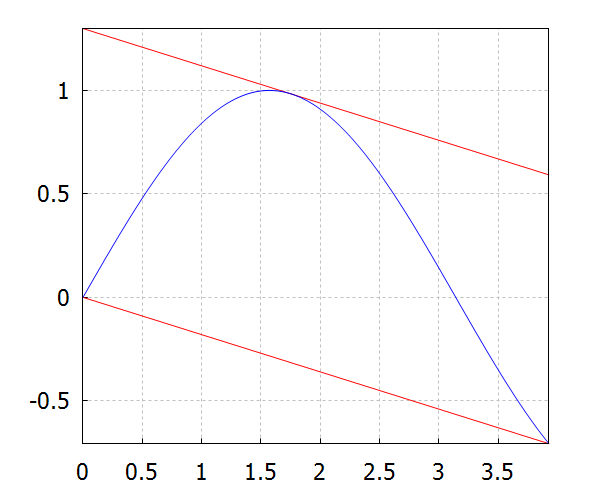
\includegraphics[scale=0.5]{Imagen17}
\end{center}
\caption{En la figura se puede ver un ejemplo con $f(x)=\sin(x)$ para $x\in \bigg[0,\dfrac{5\pi}{4}\bigg]$}
\end{figure}
\framebreak
\vspace*{-0.7cm}
\begin{block}{Teorema del valo extremo}
\begin{itemize}
\item Si $f\in C[a,b]$, entonces existe $c_1,c_2\in [a,b]$ con
$$f(c_1)\leq f(x)\leq f(c_2)$$
para $x\in[a,b]$.
\item Si además $f$ es diferenciable en $(a,b)$, entonces $c_1$ y $c_2$ son iguales a los extremos ($a$ o $b$) o los lugares donde la derivada se hace cero en $(a,b)$. 
\end{itemize}
\hyperlink{EjercicioExtremos}{\textcolor{cyan}{Enlace a ejercicio}}
\end{block}
\begin{figure}[H]
\begin{center}
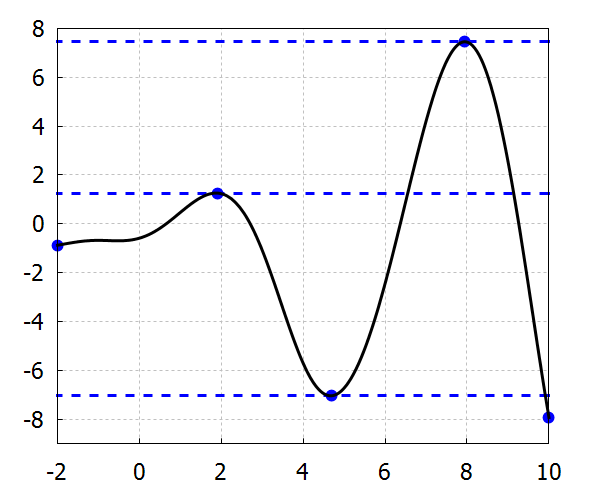
\includegraphics[scale=0.4]{Imagen18}
\end{center}
\caption{Se puede apreciar en el ejemplo, que el máximo de la función se alcanza en un lugar donde la derivada es cero y el mínimo en el extremo derecho.}
\end{figure}
\framebreak
\begin{block}{Teorema del valor intermedio}
Si $f\in C[a,b]$ y $K$ es cualquier número entre $f(a)$ y $f(b)$, entonces existe un número $c$ en $(a,b)$ para el cual $f(c)=K$.
\end{block}
\hyperlink{EjercicioIntermedio}{\textcolor{cyan}{Enlace a ejercicio}}
\begin{figure}[H]
\begin{center}
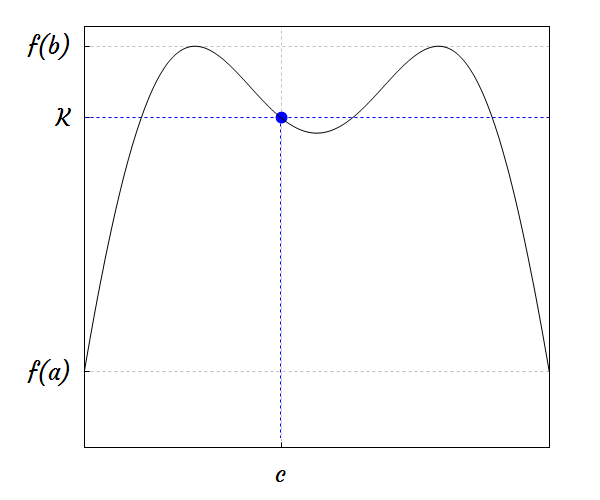
\includegraphics[scale=0.7]{Imagen19}
\end{center}
\end{figure}
\framebreak
Se define $C^n[a,b]=\{f:[a,b]\rightarrow \mathbb{R}| f,f',\cdots,f^{(n)}\text{ son continuas en }[a,b]\}.$
\begin{block}{Teorema de Taylor}
Supong que:
\begin{itemize}
\item $f\in C^n[a,b]$.
\item $f^{(n+1)}$ esta definida en $[a,b]$.
\item $x_0\in[a,b]$.
\end{itemize} 
Entonces, para cada $x\in[a,b]$, existe $\xi(x)\in (x_0,x)$ (si $x>x_0$ y $\xi(x)\in(x,x_0)$ en el otro caso)  tal que: 
\begin{itemize}
\item $f(x)=P_n(x)+R_n(x)$ donde
\item $P_n(x)=\displaystyle \sum_{k=0}^{n}\dfrac{f^{(k)}(x_0)}{k!}(x-x_0)^k$ y
\item $R_n(x)=\dfrac{f^{(n+1)}(\xi(x))}{(n+1)!}(x-x_0)^{(n+1)}$.
\end{itemize}
\end{block}
\hyperlink{EjercicioTaylor}{\textcolor{cyan}{Enlace a ejercicio}}
\end{frame}
\section{Raíces de ecuaciones}
\begin{frame}[allowframebreaks,fragile]{Raíces de ecuaciones}
\begin{figure}[H]
\begin{center}
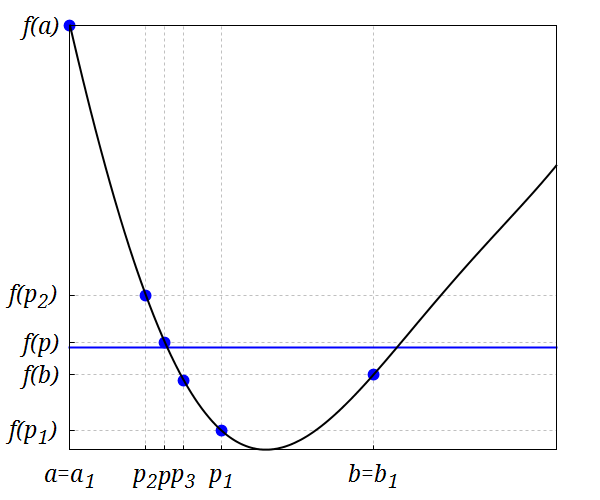
\includegraphics[scale=0.7]{Imagen20}
\end{center}
\caption{\textbf{Método de Bisección: }En la figura se muestra el mécanismo de la bisección.}
\end{figure}
\begin{lstlisting}[caption=''Método de Bisección'',style=mystyle,language=octave,numbers=left]
function x=Biseccion(f,a,b,TOL,N0)
  i=1;FA=f(a);
  while(i<=N0)
    p=a+(b-a)/2;
    FP=f(p);
    if(FP==0 || (b-a)/2<TOL)
      x=p;
      break;
    endif
    i=i+1;
    if(FA*FP>0) 
      a=p;
      FA=FP;
    else
      b=p;  
    endif
  endwhile
  if(i>N0)
    x=inf;
  endif
endfunction
\end{lstlisting}
\begin{block}{Teorema de convergencia del método de bisección}
Supongamos que $f\in C[a,b]$ y $f(a)f(b)<0$. El método de bisección genera una sucesión $\{p_n\}$ que aproxima a un cero de $p$ de $f$, tal que:
$$|p_n-p|\leq \dfrac{b-a}{2^n}.$$
\hyperlink{EjercicioBiseccion}{\textcolor{cyan}{Enlace a ejercicio}}
\end{block}
\textcolor{red}{
\indent Primero note que $p\in [a_n,b_n]$ (teorema del valor intermedio), entonces $$|p-(a_n+b_n)/2|\leq(b_n-a_n)/2.$$ De esto se tiene que:
\begin{align*}
|p_n-p|=&|(a_n+b_n)/2-p|\\
\leq & \dfrac{b_n-a_n}{2}\\
\leq & \dfrac{1}{2}\dfrac{b-a}{2^{n-1}} (\text{ inducción}: b_n-a_n\leq \dfrac{b-a}{2^{n-1}})\\
=& \dfrac{b-a}{2^n.}
\end{align*}
}
\end{frame}